\section{Análisis de sensibilidad}


\begin{figure}
\centering
\centering
\begin{subfigure}[b]{0.65\textwidth}
     \centering
     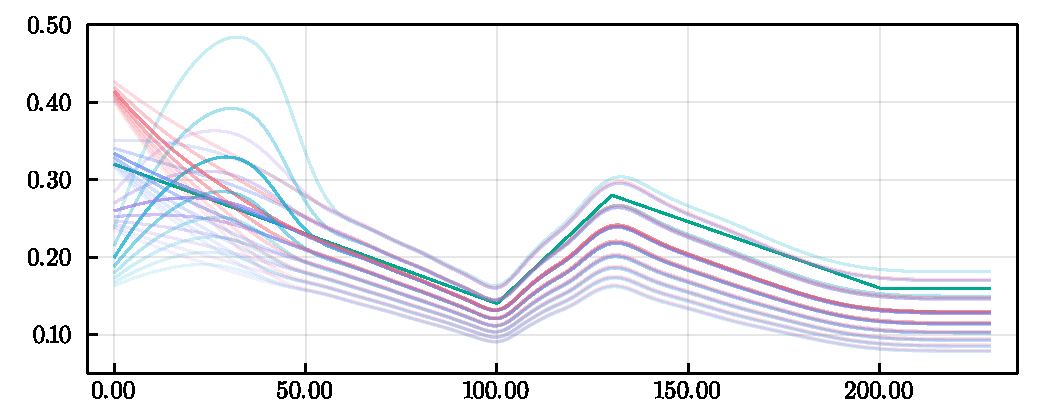
\includegraphics[width=\textwidth]{img/resultados/synth/sensibeta1-2_0-3_3-4_alpha0-15_0-1_0-45high1b2real1-88_gereal0-1961_gireal0-1389_acov0-8_aini0-27675_gcov0-05gamma_e_0-1724_gamma_i_0-1220_beta_2_2-0000.pdf}
\end{subfigure}
\hfill
\begin{subfigure}[b]{0.3\textwidth}
 \centering
\scalebox{0.7}{
\begin{tikzpicture}
	\begin{pgfonlayer}{nodelayer}
		\node [style=none] (0) at (1, 2) {};
		\node [style=none] (1) at (2.5, 2) {};
		\node [style=none] (2) at (1, 1.5) {};
		\node [style=none] (3) at (2.5, 1.5) {};
		\node [style=none] (4) at (1, 1) {};
		\node [style=none] (5) at (2.5, 1) {};
		\node [style=none] (6) at (1, 0.5) {};
		\node [style=none] (7) at (2.5, 0.5) {};
		\node [style=none] (8) at (3, 2) {$0.15$};
		\node [style=none] (9) at (3, 1.5) {};
		\node [style=none] (10) at (3, 1.5) {};
		\node [style=none] (11) at (3, 1.5) {$0.25$};
		\node [style=none] (12) at (3, 1) {};
		\node [style=none] (13) at (3, 1) {$0.35$};
		\node [style=none] (15) at (3, 0.5) {$0.45$};
		\node [style=none] (17) at (2, 2.5) {Condición inicial $\alpha_0$};
		\node [style=none] (19) at (5, 2.75) {$\beta_{\textrm{ext}}$};
		\node [style=none] (21) at (2, -0.25) {$\beta_{\text{ext}}$ solución real};
		\node [style=none] (22) at (1, -0.75) {};
		\node [style=none] (23) at (2.5, -0.75) {};
		\node [style=none] (24) at (3, -0.75) {};
		\node [style=none] (25) at (3, -0.75) {$1.88$};
		\node [style=none] (26) at (4, 2.25) {};
		\node [style=none] (27) at (5.5, 2.25) {};
		\node [style=none] (28) at (4, 1.75) {};
		\node [style=none] (29) at (5.5, 1.75) {};
		\node [style=none] (30) at (4, 1.25) {};
		\node [style=none] (31) at (5.5, 1.25) {};
		\node [style=none] (32) at (4, 0.75) {};
		\node [style=none] (33) at (5.5, 0.75) {};
		\node [style=none] (34) at (4, 0.25) {};
		\node [style=none] (35) at (5.5, 0.25) {};
		\node [style=none] (36) at (4, -0.25) {};
		\node [style=none] (37) at (5.5, -0.25) {};
		\node [style=none] (38) at (4, -0.75) {};
		\node [style=none] (39) at (5.5, -0.75) {};
		\node [style=none] (40) at (4, -1.25) {};
		\node [style=none] (41) at (5.5, -1.25) {};
		\node [style=none] (42) at (6, 2.25) {$1.2$};
		\node [style=none] (43) at (6, 1.75) {$1.5$};
		\node [style=none] (44) at (6, 1.25) {$1.8$};
		\node [style=none] (45) at (6, 0.75) {$2.1$};
		\node [style=none] (46) at (6, 0.25) {$2.4$};
		\node [style=none] (47) at (6, -0.25) {$2.7$};
		\node [style=none] (48) at (6, -0.75) {$3.0$};
		\node [style=none] (49) at (6, -1.25) {$3.3$};
		\node [style=none] (50) at (0, 3.25) {};
		\node [style=none] (51) at (6.5, 3.25) {};
		\node [style=none] (52) at (6.5, -1.75) {};
		\node [style=none] (53) at (0, -1.75) {};
		\node [style=none] (54) at (0, -2.25) {};
		\node [style=none] (55) at (6.5, -2.25) {};
	\end{pgfonlayer}
	\begin{pgfonlayer}{edgelayer}
		\draw [style={a0_1}] (0.center) to (1.center);
		\draw [style={a0_2}] (2.center) to (3.center);
		\draw [style={a0_3}] (4.center) to (5.center);
		\draw [style={a0_4}] (6.center) to (7.center);
		\draw [style=real] (22.center) to (23.center);
		\draw [style=beta1] (26.center) to (27.center);
		\draw [style=beta2] (28.center) to (29.center);
		\draw [style=beta3] (30.center) to (31.center);
		\draw [style=beta4] (32.center) to (33.center);
		\draw [style=beta5] (34.center) to (35.center);
		\draw [style=beta6] (36.center) to (37.center);
		\draw [style=beta7] (38.center) to (39.center);
		\draw [style=beta8] (40.center) to (41.center);
		\draw (50.center) to (51.center);
		\draw (51.center) to (52.center);
		\draw (52.center) to (53.center);
		\draw (53.center) to (50.center);
	\end{pgfonlayer}
\end{tikzpicture}

}
\end{subfigure}
\caption[Sensibilidad ante riesgo exterior.]{Sensibilidad ante riesgo exterior.} \label{fig:legend-sensi-b}
\end{figure}

